\documentclass[12pt, titlepage]{article}
\usepackage{xcolor} % for different colour comments

%% Comments
\newif\ifcomments\commentstrue

\ifcomments
\newcommand{\authornote}[3]{\textcolor{#1}{[#3 ---#2]}}
\newcommand{\todo}[1]{\textcolor{red}{[TODO: #1]}}
\else
\newcommand{\authornote}[3]{}
\newcommand{\todo}[1]{}
\fi

\newcommand{\wss}[1]{\authornote{magenta}{SS}{#1}}
\newcommand{\ds}[1]{\authornote{blue}{DS}{#1}}

%% Graphics
\usepackage{float}
\usepackage{caption}
\usepackage{graphicx}
\usepackage{fullpage}
\usepackage[round]{natbib}
\usepackage{multirow}
\usepackage{booktabs}
\usepackage{graphicx}
\usepackage{float}
\graphicspath{ {Images/} }

\begin{document}

\title{Smart Waiter System Architecture} 
\author{Meraj Patel \#1137491 \\ Pavneet Jauhal \#1149311\\ Shan Perera \#1150394}
\date{\today}
\maketitle

\tableofcontents 

\listoffigures

\listoftables

\section{Introduction}

\subsection{Purpose}

\subsection{Description}

\subsection{Scope}

\section{Overview}

\subsection{Design Principals}
\subsubsection{Information Hiding}

\subsubsection{Single Responsibility Principal}
This principal states every class should have responsibility of a single action within the software architecture. This action shall be encompassed in a class. Doing so will keep each process action separate allowing better organization. 

\subsection{Document Structure}
This document structure is based on the general software design document template. This document provides a general overview of purpose, description and scope of Smart Waiter. It then provides a detailed review of system architecture and data design in decomposed components. Lastly, the document provides project schedule. 

\subsection{Revision History}

\begin{table}[H]
\begin{tabular}{|c|c|}
\hline
\textbf{Date}  & \textbf{Comments} \\ \hline
January 11, 2016 &  first draft. \\ 
\hline
\end{tabular}
\caption{Revision History Table}
\end{table}

\section{Control Flow Diagram}
Below is a high level overview of Smart Waiter operation. The operation is decomposed into components which is introduced in this section and will be thoroughly explained in the following sections. 


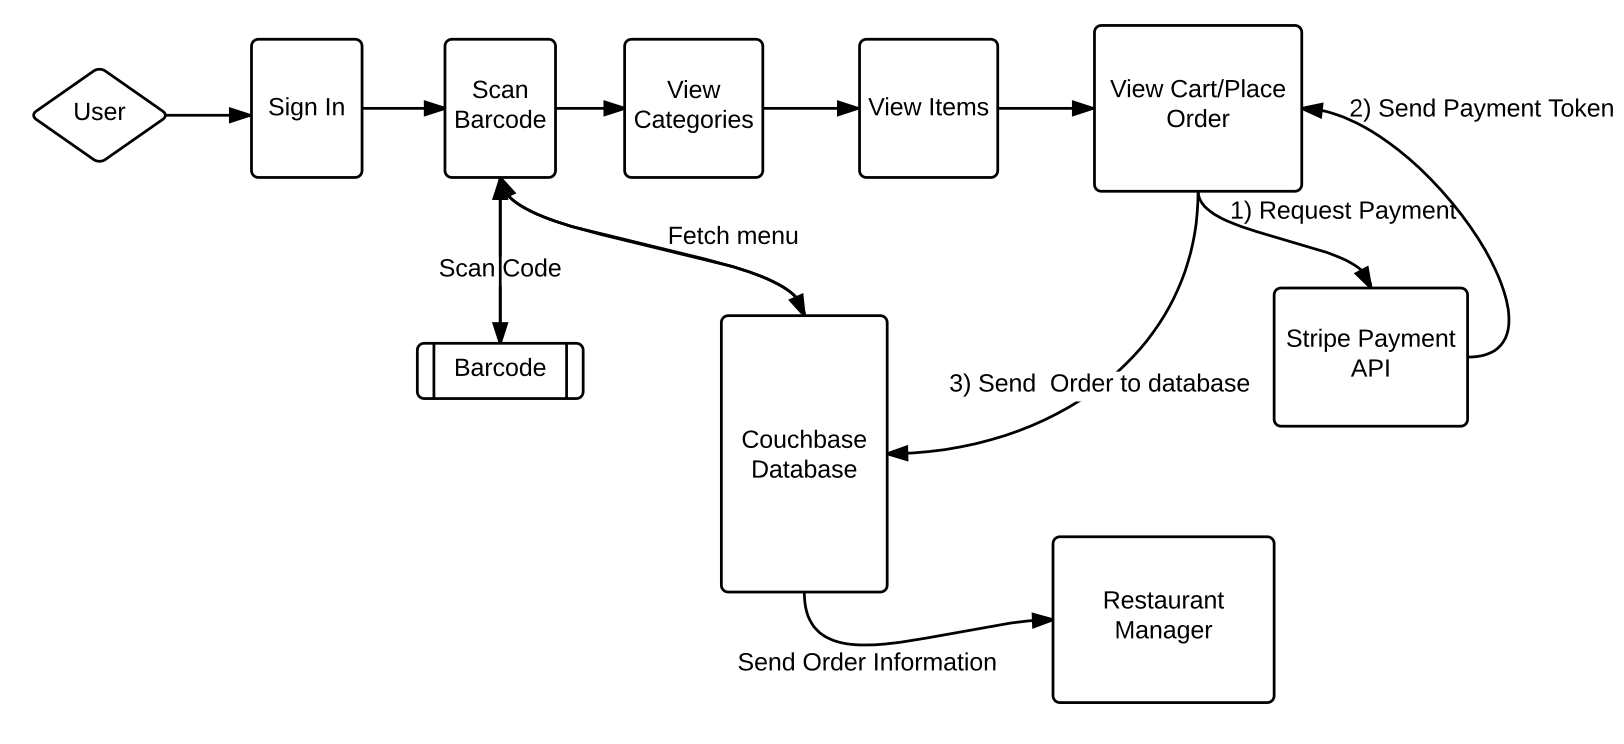
\includegraphics[width=150mm,scale=0.5]{OverallOperation.png}

\section{Module Decomposition}


\subsection{Ordering Class Structure}
There are three primary classes used to hold all vital information regarding menu information. These are: MenuCategories, MenuItems and User. In correspondence with single responsibility principal, each class is encompasses a single purpose. This purpose and how classes correlate with each other is described below. 

\subsubsection{MenuCategories Class}
This class purpose is to store menu category information of a restaurant menu. This entails category name, picture and a reference to category items. To do so, there are three main variables used within this class to hold this information: 

\begin{description}
  \item[categoryName:] Stores category name in the form of String
  \item[picURL:] Stores URL of category picture
  \item[categoryItems:] Stores an array of objects that reference MenuItems class
\end{description}


This class is instantiated and called upon when a user successfully scans a barcode. The JSON response acquired from the database is parsed, and information related to menu categories is stored appropriately within this class. The application uses this class to display category information when "Menu Categories" page is spawned (please see section 5.1.1 to view picture).

\subsubsection{MenuItems Class}
This class purpose is to store menu item information of a restaurant menu. This means, item name, price and description. Thee main variables are used within this class to hold this information.

\begin{description}
  \item[itemName:] Stores item name
  \item[itemPrice:] Stores item price
  \item[itemDetail:] Stores description of item
\end{description}

Objects of this class are instantiated from the MenuCategories class. By successfully scanning the barcode and parsing the JSON response, MenuItem objects are instantiated and used to save item details. These objects are held within categoryItems list seen in Menu Categories class. This application uses this class to display item information of a category when "Menu Items" page is spawned (please see section 5.1.2 to view picture). These objects are also used in reference to items the user would like to order. This is thoroughly discussed in the proceeding section.  

\subsubsection{User Class}
User class is used to store menu item a user would like to order. For now, there is only one important variable to consider: 

 \begin{description}
  \item[userItem:] an array that stores objects of MenuItems class. This is used to save menu items a user would like to order.
\end{description}

Only one object is instantiated through the life time of this application. This object represents the user cart of menu items he/she would like to order. This object is called upon when a user decides to add an item to their cart. When this occurs, a copy of the MenuItem object is saved within the userItem variables. This way, there is a list maintained to hold all item a user would like to order. When a user confirms and sends their order, the item information is extracted from userItem list, formatted into a JSON request and send back to the database for further processing. Having this class implemented allows extendibility in the future, as all vital information pertaining to a user can be stored within the class (for example, user settings). 


\subsection{Camera Structure}
There is one main function related to the Camera structure: onActivityResult. The camera is used to read QR codes, which contain the location of where the menu data is stored in relation to the current restaurant. The QR codes are read using an embedded version of the ZXing library. When the application starts, a ZXing specific variable (IntentIntegrator) is initialized, when the user clicks the "Scan QR Code" button on the first screen, the Camera is initialized. 

\subsubsection{Design Principles}
This component follows the Single Responsibility and the Information Hiding principle.  

\begin{description}
	\item[Single Responsibility:] The responsibility of this component is to capture and parse QR code data. If this component had to be changed, it would only affect the camera functionality of the application, and not other components like the menu or accounts.
	\item[Information Hiding:] The camera component is separate from every other component of this application. If any changes were to be made to the camera application, it will not affect the other components of the application. However, it is unlikely that there will be any changes applied to this component of the application.
\end{description}

\subsubsection{onActivityResult}
This function uses an integrated version of the ZXing library to scan QR codes. After the camera is initialized, the application waits for the user to pass a QR code, this is done by taking a picture of the QR code with the camera. The function onActivityResult is called as soon as a QR code is passed. It takes, as input a requestCode, resultCode, and the current intent: 

\begin{description}
  \item[requestCode:] Used to parse the QR code 
  \item[resultCode:] Used to parse the QR code 
  \item[intent:] Gives the current intent, used to parse the QR code
\end{description}

Using the given input, the function parses and gets the contents of the QR code that was passed to the function using the ZXing function parseActivityResult. The information stored in the QR code is then saved to a local variable to be used by the other components of the application.

\subsubsection{Module Decomposition}
Module: onActivityResult
\begin{description}
	\item[Secret:]How the QR code is parsed and read
	\item[Service:] Parses and gets the content of the QR code
\end{description}

\subsection{Accounts Structure}
There are 3 main classes related to the Accounts structure: User, Card, and Stripe. Accounts are used to associate a user identifier for transactions and for storing a user's credit card information securely. Credit card information transfer and storage uses Stripe API. This reduces the burden on the developers, since we can use an established API that follows the restrictions applied by credit card companies, and handles the secure transfer of sensitive information, rather than developing an efficient and secure system ourselves.

\subsubsection{Design Principles}
This component follows the Single Responsibility and the Information Hiding principle.  

\begin{description}
	\item[Single Responsibility:] The responsibility of this component is to securely store a user's credit card information for use in account transactions. If this component had to be changed, it would only affect the accounts functionality of the application, and not other components like the menu or camera.
	\item[Information Hiding:] The accounts component is separate from every other component of this application. If any changes were to be made to the accounts module, it will not affect the other components of the application.
\end{description}

\subsubsection{User Class}
This class creates a structure for storing a user's account information and general details. The User class has 7 field variables for storing the user's general information. The field variables include: username, password, firstName, lastName, billingAddress, postalCode, phoneNumber

\begin{description}
  \item[username:] Used as an identifier for the user 
  \item[password:] Used for logging into the user's account 
  \item[firstName:] First name of the user, used for the billing address
  \item[lastName:] Last name of the user, used for the billing address
  \item[billingAddress:] User's home address, used for billing address
  \item[postalCode:] User's home address, used for billing address
  \item[phoneNumber:] User's phone number, used if we need to get in touch with the user
\end{description}

\subsubsection{Card Class}
This class creates a structure for storing a user's credit card information. The Card class has 4 field variables, which include: cardNumber, cardExpMonth, cardExpYear, cardCVC.

\begin{description}
  \item[cardNumber:] Stores the 16 digit credit card number 
  \item[cardExpMonth:] Stores the 2 digit expiry month 
  \item[cardExpYear:] Stores the 4 digit expiry year
  \item[cardCVC:] Stores the 3 digit CVC code, stored to prevent fraud
\end{description}

\subsubsection{Stripe}
This method is used to securely send credit card information to the Stripe server, the Stripe servers then sends a token that can be used to charge the user's credit card. An instance of the Card class is created using the user's credit card information, and a token is created
using the card and the application's Stripe API key. The token is sent to the server, Stripe then returns a token that can be used to charge the user's credit card. The transaction parameters are passed to the charge function, which is then used to accurately charge the user's card.
The parameters include: amount, currency, source, and description.
  
\begin{description}
  \item[amount:] An integer value of the amount to be charged to the user's credit card in cents.
  \item[currency:] A string value of the type of currency to be charged, for our application, we will use Canadian dollars (CAD) 
  \item[source:] A string value of Stripe token retrieved from the Stripe servers 
  \item[description:] A string value containing the description of the charge to the user's credit card.
\end{description}

\subsubsection{Module Decomposition}
Module: chargeParams
\begin{description}
	\item[Secret:]How the user's credit card is charged accurately
	\item[Service:] Charges the user's credit card based on the parameters passed.
\end{description}

\section{Traceability Matrix}
Below describes how our decomposed modules relate to requirements specified in SRS
\begin{table}[H]
\centering
\begin{tabular}{p{0.2\textwidth} p{0.6\textwidth}}
\toprule
\textbf{Req.} & \textbf{Modules}\\
\midrule
R1 & Camera Structure\\
R2 & Accounts Structure\\
R3 & Accounts Structure\\
R6 & Ordering Class Structure\\
R7 & Ordering Class Structure\\
R9 & Ordering Class Structure\\
R13 & Accounts Structure \\
R14 & Accounts Structure\\
R15 & Ordering Class Structure\\
R16 & Ordering Class Structure\\
R18 & Ordering Class Structure\\
R19 & Ordering Class Structure\\
\bottomrule
\end{tabular}
\caption{Trace Between Requirements and Modules}
\label{TblRT}
\end{table}

\section{Likely Future Changes}
\subsection{Anticipated Changes}
\begin{description}
  \item[Database:] Consolidation of both databases (for menu items, and orders)
  \item[Accounts:] Switch to self made account system rather then using Facebook API as it may have compatibility issues
 \end{description}
 
\subsection{Extra Design Features}
\begin{description}
  \item[User Preferences:] Make more use of User class by providing the user the ability to store preferences. Eg, food allergies, past meals
\end{description}


\end{document}
